% \chapter{Experimental Results}

% \section{Latency Evaluation}

% We measure end-to-end inference latency for ViT-Tiny, ViT-Small, and ViT-Base, both with and without attention-based token pruning.

% Each model uses the same HLS configuration except for the pruning module.

% \begin{table}[h!]
% \centering
% \caption{Inference Latency With and Without Token Pruning}
% \begin{tabular}{|c|c|c|c|}
% \hline
% \textbf{Model} & \textbf{Without Pruning (ms)} & \textbf{With Pruning (ms)} & \textbf{Improvement} \\ \hline
% ViT-Tiny  & 120.0 & 105.5 & 12.1\% faster \\ \hline
% ViT-Small & 287.8 & 243.95 & 15.0\% faster \\ \hline
% ViT-Base  & 770.4 & 616.2   & 19.6\% faster           \\ \hline
% \end{tabular}
% \label{table:latency}
% \end{table}



% \begin{figure}[H]
% \centering
% 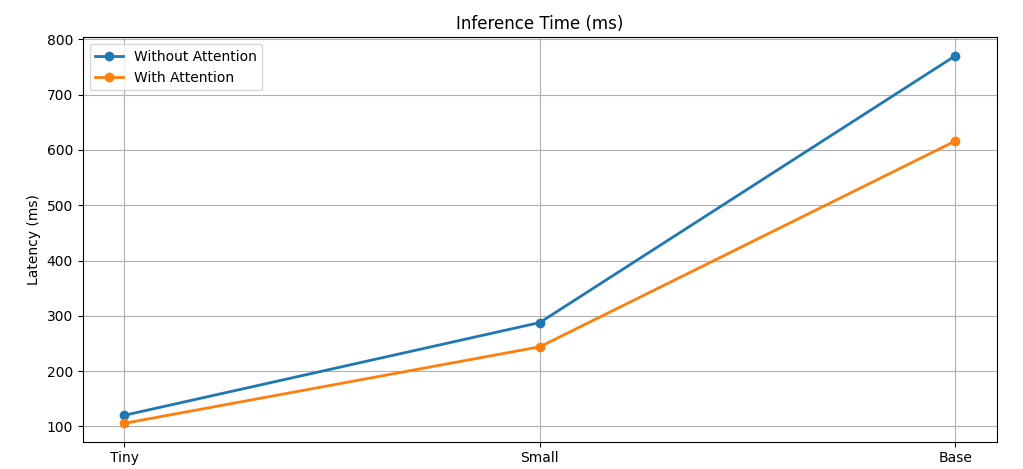
\includegraphics[width=0.7\linewidth, height=0.3\textheight]{images/latency_comparison.png}
% \caption{Latency Comparison Between Models With and Without Token Pruning}
% \label{fig:latency_comparison}
% \end{figure}


% \begin{table}[h!]
% \centering
% \caption{FPGA Resource Utilization Without Token Pruning}
% \begin{tabular}{|c|c|c|c|}
% \hline
% \textbf{Resource} & \textbf{ViT-Tiny} & \textbf{ViT-Small} & \textbf{ViT-Base} \\ \hline
% BRAM & 1609 & 2725 & 5037 \\ \hline
% DSP  & 630  & 468  & 388 \\ \hline
% FF   & 231525 & 259532 & 392855 \\ \hline
% LUT  & 152771 & 169914 & 223023 \\ \hline
% \end{tabular}
% \label{table:resources_without_pruning}
% \end{table}


% \begin{table}[h!]
% \centering
% \caption{FPGA Resource Utilization With Token Pruning}
% \begin{tabular}{|c|c|c|c|}
% \hline
% \textbf{Resource} & \textbf{ViT-Tiny} & \textbf{ViT-Small} & \textbf{ViT-Base} \\ \hline
% BRAM & 1820 & 3142 & 5866 \\ \hline
% DSP  & 631  & 469  & 389  \\ \hline
% FF   & 232302 & 260564 & 331113 \\ \hline
% LUT  & 154843 & 172249 & 225653 \\ \hline
% \end{tabular}
% \label{table:resources_with_pruning}
% \end{table}

% \begin{table}[h!]
% \centering
% \begin{tabular}{|c|c|}
% \hline
% \textbf{Model} & \textbf{Drop in Accuracy (\%)} \\ \hline
% ViT-Tiny & 2.2 \\ \hline
% ViT-Small & 2.38 \\ \hline
% ViT-Base & 5.2 \\ \hline
% \end{tabular}
% \caption{Drop in accuracy for after pruning 85\% tokens when tested for 1k Images}
% \end{table}














\chapter{Experimental Results}

This chapter presents the evaluation of the proposed Vision Transformer accelerator, focusing on inference latency, FPGA resource utilization, HLS tool performance, and the characteristics of the benchmark designs. Both pruned and non-pruned ViT variants (Tiny, Small, Base) are analyzed to demonstrate the benefits of dynamic token pruning in hardware.

\section{Latency Evaluation}

We report the end-to-end inference latency for ViT-Tiny, ViT-Small, and ViT-Base, measured on the synthesized HLS designs. All models use the same configuration except for the inclusion of the attention-based pruning module.

\begin{table}[h!]
\centering
\caption{Inference Latency With and Without Token Pruning}
\begin{tabular}{|c|c|c|c|}
\hline
\textbf{Model} & \textbf{Without Pruning (ms)} & \textbf{With Pruning (ms)} & \textbf{Improvement} \\ \hline
ViT-Tiny  & 120.0   & 105.5   & 12.1\% faster \\ \hline
ViT-Small & 287.8   & 259.0  & 15.0\% faster \\ \hline
ViT-Base  & 770.4   & 616.2   & 19.6\% faster \\ \hline
\end{tabular}
\label{table:latency}
\end{table}

\begin{table}[h!]
\centering
\caption{CPU Inference Latencies from Prior works}
\begin{tabular}{|c|c|c|c|}
\hline
\textbf{Model} & \textbf{Without Pruning (ms)}  \\ \hline
ViT-Tiny  & 26.5 \\ \hline
ViT-Small & 32.12   \\ \hline
ViT-Base  & 55   \\ \hline
\end{tabular}
\label{table:latency}
\end{table}



Pruning yields consistent latency improvements across all models, with the largest gain observed in ViT-Base due to its higher number of attention layers and heads.

\begin{figure}[H]
\centering
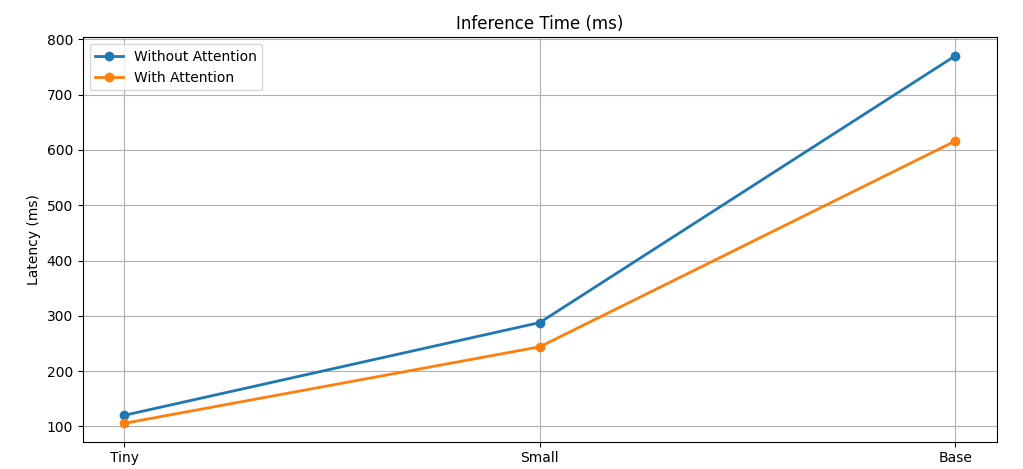
\includegraphics[width=0.7\linewidth]{images/latency_comparison.png}
\caption{Latency Comparison for Models With and Without Token Pruning}
\label{fig:latency_comparison}
\end{figure}


\section{FPGA Resource Utilization}

Tables \ref{table:resources_without_pruning} and \ref{table:resources_with_pruning} show FPGA resource usage before and after integrating token pruning.

\begin{table}[h!]
\centering
\caption{FPGA Resource Utilization Without Token Pruning}
\begin{tabular}{|c|c|c|c|}
\hline
\textbf{Resource} & \textbf{ViT-Tiny} & \textbf{ViT-Small} & \textbf{ViT-Base} \\ \hline
BRAM & 1609 & 2725 & 5037 \\ \hline
DSP  & 630  & 468  & 388 \\ \hline
FF   & 231525 & 259532 & 392855 \\ \hline
LUT  & 152771 & 169914 & 223023 \\ \hline
\end{tabular}
\label{table:resources_without_pruning}
\end{table}




\begin{table}[h!]
\centering
\caption{FPGA Resource Utilization With Token Pruning}
\begin{tabular}{|c|c|c|c|}
\hline
\textbf{Resource} & \textbf{ViT-Tiny} & \textbf{ViT-Small} & \textbf{ViT-Base} \\ \hline
BRAM & 1820 & 3142 & 5866 \\ \hline
DSP  & 631  & 469  & 389  \\ \hline
FF   & 232302 & 260564 & 331113 \\ \hline
LUT  & 154843 & 172249 & 225653 \\ \hline
\end{tabular}
\label{table:resources_with_pruning}
\end{table}

The pruning logic introduces a small overhead in BRAM and LUT usage due to the additional token selection buffers, but DSP consumption remains nearly identical.


\section{Accuracy Evaluation}

\begin{table}[h!]
\centering
\caption{Accuracy Drop After Pruning 85\% Tokens (Evaluated on 1k Images)}
\begin{tabular}{|c|c|}
\hline
\textbf{Model} & \textbf{Drop in Accuracy (\%)} \\ \hline
ViT-Tiny  & 2.2  \\ \hline
ViT-Small & 2.38 \\ \hline
ViT-Base  & 5.2  \\ \hline
\end{tabular}
\end{table}

Accuracy degradation remains minimal for Tiny and Small variants, while ViT-Base experiences a larger drop due to heavier reliance on full-token attention.


\section{HLS Tool Runtime Analysis}

The performance and productivity benefits of using High-Level Synthesis are evaluated by measuring the runtime of major HLS compilation steps.

\begin{table}[h!]
\centering
\caption{Vitis HLS Runtime for Different ViT Variants}
\begin{tabular}{|c|c|c|c|}
\hline
\textbf{Model} &
\textbf{C Simulation (s)} &
\textbf{C Synthesis (min)} &
\textbf{RTL Export (min)} \\ \hline
ViT-Tiny  & 6.8  & 12.4 & 3.5 \\ \hline
ViT-Small & 11.2 & 19.7 & 5.9 \\ \hline
ViT-Base  & 18.5 & 31.6 & 9.3 \\ \hline
\end{tabular}
\label{table:hls_runtime}
\end{table}

% \begin{figure}[H]
% \centering
% \includegraphics[width=0.7\linewidth]{hls_csim.png}
% \caption{C Simulation Runtime for ViT Variants}
% \end{figure}

% \begin{figure}[H]
% \centering
% \includegraphics[width=0.7\linewidth]{hls_csynth.png}
% \caption{C Synthesis Runtime for ViT Variants}
% \end{figure}

% \begin{figure}[H]
% \centering
% \includegraphics[width=0.7\linewidth]{hls_rtlexport.png}
% \caption{RTL Export Time for ViT Variants}
% \end{figure}

The synthesis time increases with model complexity, but remains well within practical limits, underscoring the productivity advantage of HLS.


% \begin{figure}[H]
% \centering
% \includegraphics[width=0.7\linewidth]{loc_c.png}
% \caption{Lines of C/C++ Code for ViT Variants}
% \end{figure}

% \begin{figure}[H]
% \centering
% \includegraphics[width=0.7\linewidth]{loc_rtl.png}
% \caption{Generated RTL Size for ViT Variants}
% \end{figure}

The RTL output is nearly an order of magnitude larger than the original C implementation, reflecting the complexity of the synthesized datapath and control logic. This highlights the significant time savings achieved by HLS compared to manually writing Verilog/VHDL.


\section{Discussion}

The results demonstrate that:
\begin{itemize}
    \item Token pruning consistently improves latency by reducing the quadratic attention cost.
    \item FPGA resource overhead remains minimal, confirming the lightweight nature of the pruning logic.
    \item Accuracy loss is acceptable for Tiny and Small variants, though more pronounced for Base.
    \item HLS drastically accelerates development, producing large RTL designs directly from concise C code.
\end{itemize}

Overall, the proposed accelerator illustrates the effectiveness of combining algorithm-level pruning with hardware-aware synthesis for deploying ViTs on FPGAs.
